\documentclass[10pt]{beamer}
\usepackage[utf8]{inputenc}

\usepackage{multirow,rotating}
\usepackage{xcolor}
\usepackage{hyperref}
\usepackage{tikz-cd}
\usepackage{array}
\usepackage{siunitx}
\usepackage{mathtools,nccmath}%
\usepackage{etoolbox, xparse} 
\usepackage{csquotes}
\usepackage{listings}
\usepackage{qtree}
\usepackage{multicol}
\usepackage{lmodern}

\usetheme{Pittsburgh}
\usecolortheme{dolphin}

% set colors
\definecolor{myNewColorA}{RGB}{158, 27,50}
\definecolor{myNewColorB}{RGB}{158, 27,50}
\definecolor{myNewColorC}{RGB}{130,138,143} %{158, 27,50} % {130,138,143}
\definecolor{darkgreen}{rgb}{0.0, 0.5, 0.0}
\setbeamercolor*{palette primary}{bg=myNewColorC}
\setbeamercolor*{palette secondary}{bg=myNewColorB, fg = white}
\setbeamercolor*{palette tertiary}{bg=myNewColorA, fg = white}
\setbeamercolor*{titlelike}{fg=myNewColorA}
\setbeamercolor*{title}{bg=myNewColorA, fg = white}
\setbeamercolor*{item}{fg=myNewColorA}
\setbeamercolor*{caption name}{fg=myNewColorA}
\usefonttheme{professionalfonts}
\usepackage{natbib}
% \bibliographystyle{binat}
%\usepackage{filecontents} % for inline .bib file
\usepackage{hyperref}

\usepackage[ddMMyyyy]{datetime} 
\usepackage[normalem]{ulem}
%------------------------------------------------------------
% \titlegraphic{\includegraphics[height=0.75cm]{ua_eng_logo.png}} 

% logo of my university


\titlegraphic{%

\includegraphics[width=2.0cm]{ul-logo.png}
}

\setbeamerfont{title}{size=\large}
\setbeamerfont{subtitle}{size=\small}
\setbeamerfont{author}{size=\small}
\setbeamerfont{date}{size=\footnotesize}
\setbeamerfont{institute}{size=\footnotesize}
\title[]{
%Diachronic study of semantic analogies 
Tracing and visualizing diachronic semantic change using contextualized embeddings
%for (a) given language(s) across different time periods 
}%title
\subtitle{ 
Software project, group 5
}%%subtitle
\author[UL]{Averie (Ho Zoen) SO, NGO Van Duy, Scott TANKARD, Mathilde AGUIAR
}%%authors

\date[\textcolor{white}{Our title}]
{
\today{}}

\institute[]{Universit\'e de Lorraine}
% \setbeamercovered{invisible}
% \setbeamercovered{%
%   again covered={\opaqueness<1->{15}}}

%------------------------------------------------------------
%This block of commands puts the table of contents at the 
%beginning of each section and highlights the current section:
%\AtBeginSection[]
%{
%  \begin{frame}
%    \frametitle{Contents}
%    \tableofcontents[currentsection]
%  \end{frame}
%}
\AtBeginSection[]{
  \begin{frame}
  \vfill
  \centering
  \begin{beamercolorbox}[sep=8pt,center,shadow=true,rounded=true]{title}
    \usebeamerfont{title}\insertsectionhead\par%
  \end{beamercolorbox}
  \vfill
  \end{frame}
}
% ------Contents below------
%------------------------------------------------------------

% \begin{filecontents}{\jobname.bib}
% \end{filecontents}

\begin{document}

%The next statement creates the title page.
\frame{\titlepage}
\begin{frame}
\frametitle{Outline}
\tableofcontents
\end{frame}


% consider removing it if it's too redundant
% \AtBeginSection[]
% {
%   \begin{frame}
%     \frametitle{Table of Contents}
%     \tableofcontents[currentsection]
%   \end{frame}
% }

%------------------------------------------------------------
\section{Introduction}
% this section assigned to: Scott
\begin{frame}{Project formalisation}
%\begin{itemize}
%\item
\textbf{Working draft project goal proposal:}

tracing and visualizing diachronic semantic change 
using contextualized embeddings (from m-BERT),
with re-training on an array of multilingual time-segmented corpora

(With 1 model per time segment. Example: Model A: 1910 english + 1910 french.
Model B: 1920 english + 1920 french.)

Tracing: putting in relation of multiple quantified (non-binary) measurements (of semantic change).

Underlying core-core part here is: get quantified measurements of semantic change from the model (m-bert).

%\end{itemize}
\end{frame}

\begin{frame}{Extra steps and components we may add}
As first step: set-up with just 1 language, for 2 time periods. 
Later, add additional languages into the corpuses and re-train the models.

Bonuses:

+ Run experiments on multi-senses vs single-averaged sense (WITHOUT testing on different types of semantic change)

+ analyzing multiple languages in comparison to each other (e.g. evolution of Sir/Monsieur in eng/fr)

+ historical event contextualization (database...)

+ future semantic change prediction

Non-goals (explicitly excluded from project scope):

- exploring the multilinguality inside multilingual models

- doing multiple monolingual applications %(in array -- rinse-repeat, each independent from the other)

\end{frame}


\section{HistWords}
% This section is assigned to: Duy!
% https://arxiv.org/pdf/1605.09096.pdf
% https://github.com/williamleif/histwords
% In this section I'd give a harangue about the methods, the similarity measurement(?) and bla bla
% BERT word sense https://arxiv.org/pdf/2202.03612.pdf
\begin{frame}{William L. Hamilton et al. 2018}
    Publication: \textit{Diachronic Word Embeddings Reveal Statistical Laws of Semantic Change}
    \begin{itemize}
        \item Quantified semantic changes in word embeddings
        \item Experimented on 6 datasets in 4 languages: \textsc{en, zh, de, fr}
        \item Historical embeddings are aligned with Proscrutes Regression
        \item Pairwise similarity is calculated using cos-sim
    \end{itemize}
    \begin{figure}
        \centering
        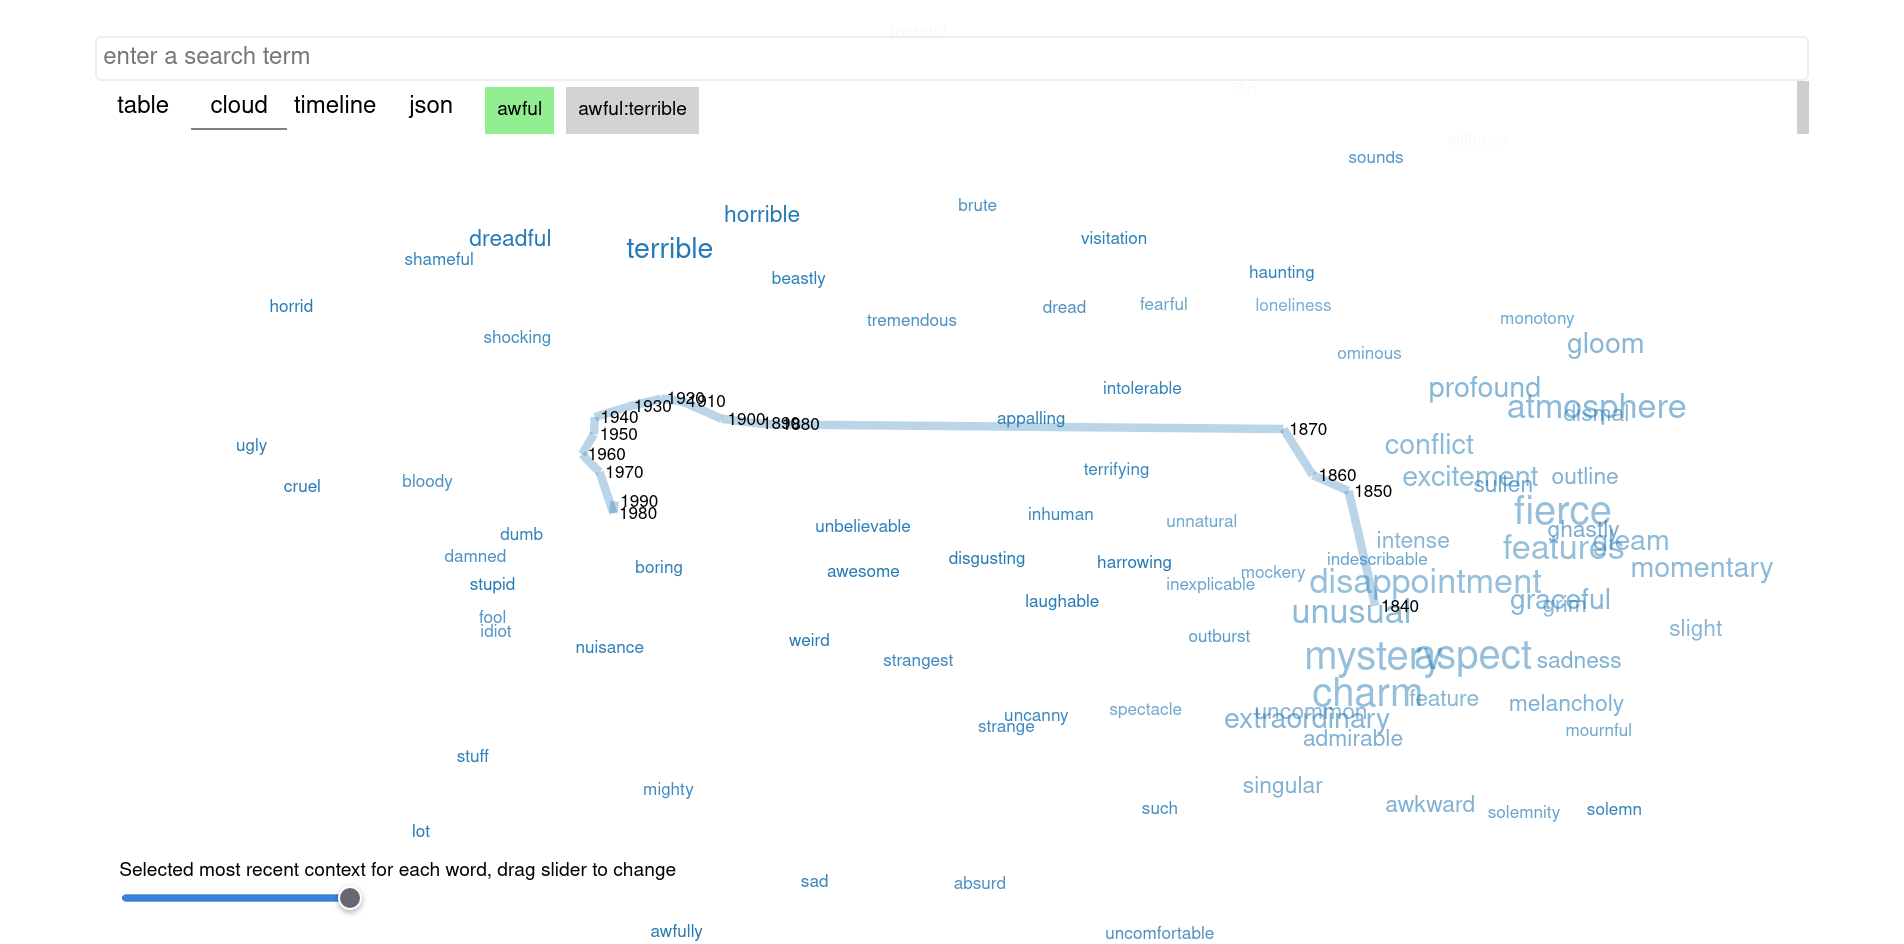
\includegraphics[width=0.6\textwidth]{figures/histwords awful 02.png}
        \caption{The illustration of \textsc{awful} meaning shifts}
        \label{fig:histwords_awful_02}
    \end{figure}
\end{frame}



\section{BERT implementation}
\begin{frame}{BERT implementation}
% This section is assigned to: Averie 
\begin{itemize}
    \item Motivation
    \begin{itemize}
        
        \item BERT is SOTA for word embeddings, but most literature in detecting semantic changes were before BERT existed (-2017)
        
        \item contextualised word embeddings can potentially better capture the various senses of the same word
        
        \item mBERT can deal with mapping embeddings across different languages
        
    \end{itemize}
    \item Challenges and proposed solutions 
    \begin{enumerate}
        \item time bias in mBERT since it is pre-trained with more contemporary data $\rightarrow$ time-specific BERT
        \item tracing multiple word senses over time $\rightarrow$ clustering
    \end{enumerate}
\end{itemize}
\end{frame}

\begin{frame}{challenge 1: time-specific mBERT}
    \begin{itemize}
        \item BERT is pre-trained on contemporary corpora (eg. Wikipedia) which often do not appropriately reflect language use in historical times. (Qiu and Xu, 2021)
        \item our attempt to alleviate this problem would be to further pre-train mBERT on time-specific corpora (unsupervised)
        \item given that we will use mBERT, we segment corpora from each language for each time period (eg. 1910 English + 1910 French, 1920 English + 1920 French..)
        \item then we train mBERT embeddings for each of these time periods multi-lingually
    \end{itemize}
\end{frame}

\begin{frame}{challenge 2: single vs multiple senses in mBERT}
\begin{itemize}
    \item single sense approach: various approaches in SemEval Task 2020 simply averaged across all contextualised embeddings of the same word 
    \item multi-sense approach: clustering, eg. Giulianelli et al, 2020 (and others)
\end{itemize}
\begin{figure}
    \centering
    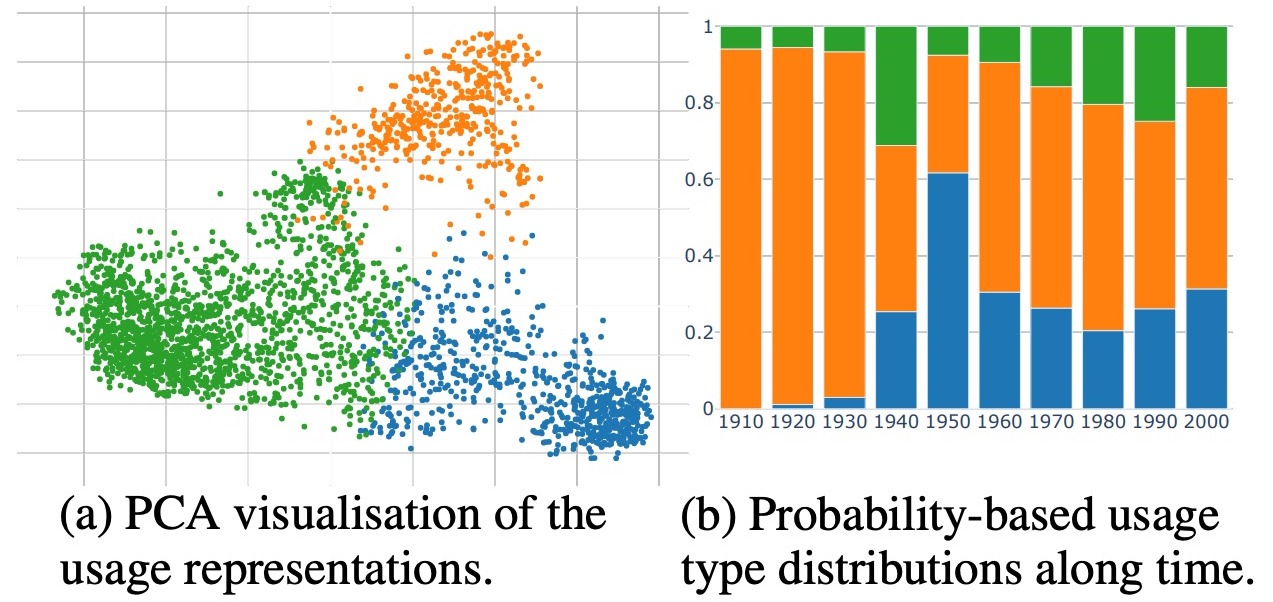
\includegraphics[width=0.6\textwidth]{giulianelli.jpeg}
    \caption{clustering and frequency distribution of senses for the word \textsc{atom}. }
\end{figure} 
\end{frame}



\begin{frame}{overall flowchart}
\begin{enumerate}
  \item obtain word embeddings from off-the-shelf mBERT, create a Usage matrix
  \begin{figure}
    \centering
    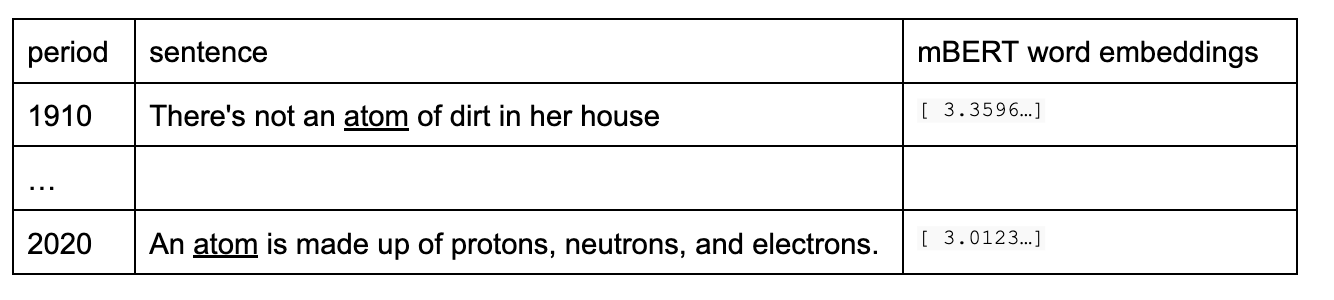
\includegraphics[width=0.8\textwidth]{step1}
  \end{figure} 
  \item clustering with k-means and silhouette score to select the optimal number of clusters and frequency distribution of word senses over time
  \begin{figure}
    \centering
    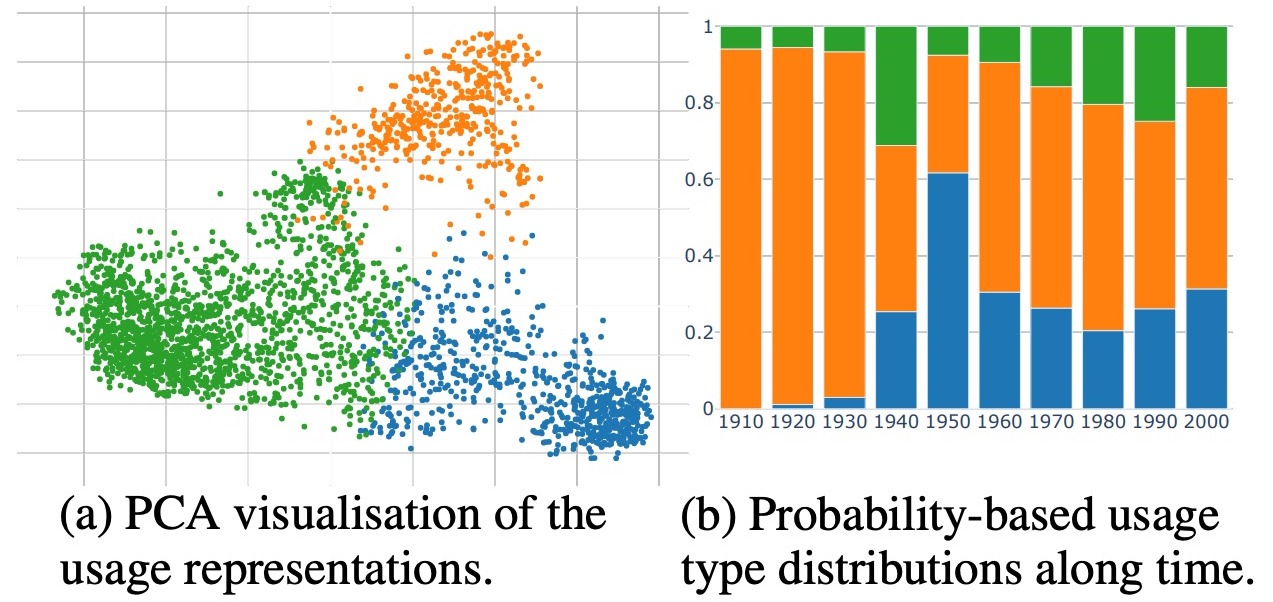
\includegraphics[width=0.6\textwidth]{giulianelli.jpeg}
\end{figure} 
  \end{enumerate}
\end{frame}

\begin{frame}{overall flowchart (cont.)}
\begin{enumerate}
    \setcounter{enumi}{2}
  \item obtain sense-tagged Usage matrix 
    \begin{figure}
    \centering
    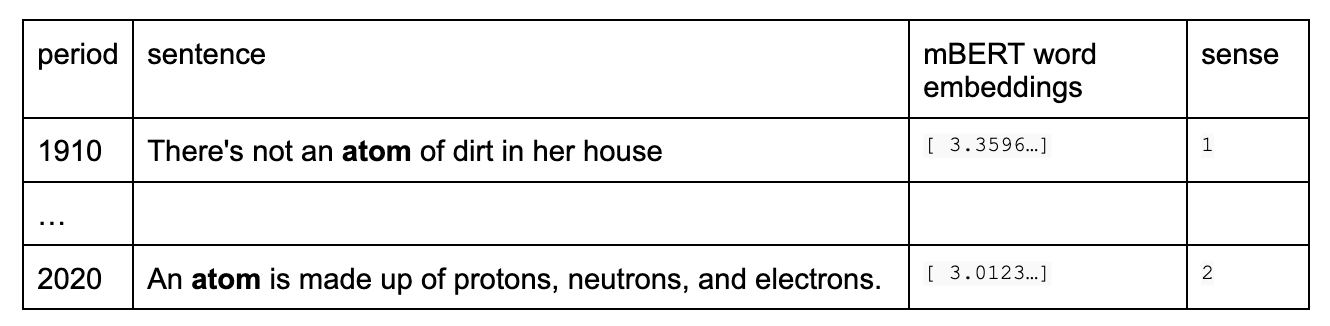
\includegraphics[width=0.8\textwidth]{step3.png}
  \end{figure} 
  \item obtain word embeddings from time-specific mBERT at each time period. in visualisation, trace the different senses
    \begin{figure}
    \centering
    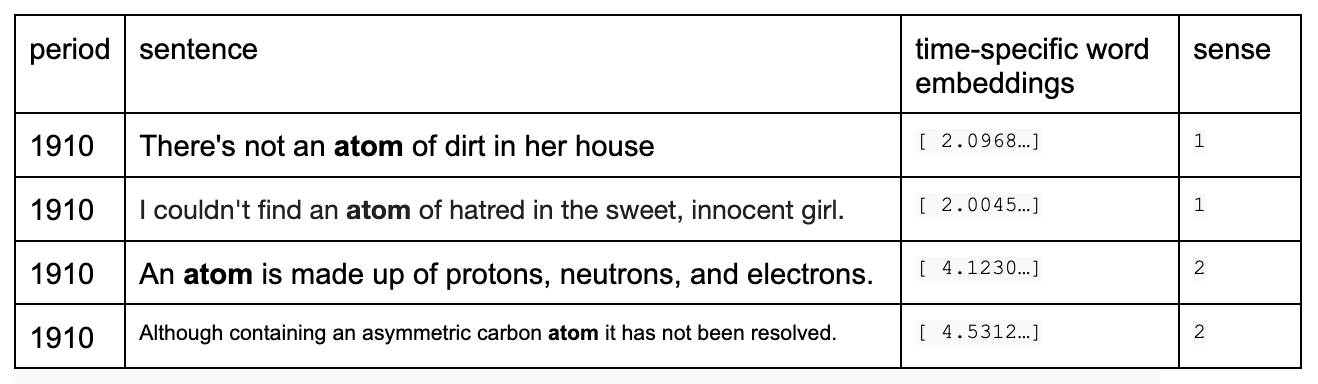
\includegraphics[width=0.8\textwidth]{step4.png}
  \end{figure} 
\end{enumerate}
\end{frame}




\section{Visualisation tools}
\begin{frame}{final visualisation}
*neighbours are made up 
    \begin{figure}
    \centering
    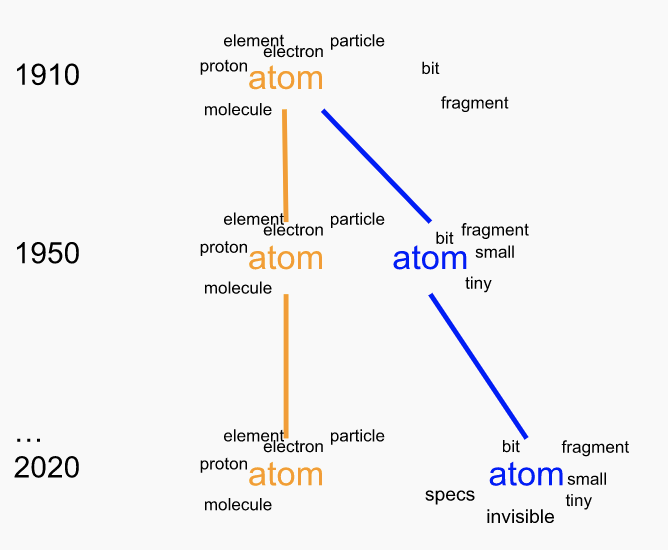
\includegraphics[width=0.8\textwidth]{final_vis.png}
  \end{figure} 
\end{frame}
\begin{frame}{Visualisation tools}
 
 2 main ideas: 
 \begin{itemize}
     \item Using the Python library Bokeh 
     $\rightarrow$ Producing a simple cluster-like graph 
 \end{itemize}
 
 \begin{itemize}
     \item Using the Stardog API $\rightarrow$ representation of the RDF graph where an entity is the meaning of linked to its translation in several languages
 \end{itemize}
     
\end{frame}

%\section{Future work}
%\subsection{Predicting}
%\subsection{Historical Events}


%\section{Conclusion}
% this section assigned to: 
%\begin{frame}{Conclusions and next steps}
%\begin{itemize}
    
    %\item Summary

    %\item Next steps
    
    %\item Remaining questions
    
%\end{itemize}
%\end{frame}

\begin{frame}{Timeline}
\begin{itemize}
    
    \item end of November: 
    understanding how to trace multiple senses in BERT; 
    obtain corpora; 
    further pre-train mBERT on two different periods of multilingual data; 
    get program to generate quantified measurements of semantic change out of mBERT;
    prototype visualisation component.
    
    \item Mid-December: 
    evaluation with existing benchmark and on historical events; 
    finish implementing solution to the multiple senses problem 
    
    \item End of December: finish training on all the time periods

    \item Rest of January: writing report


\end{itemize}
\end{frame}


%\section*{Resources}  
%\begin{frame}[allowframebreaks]
%        \frametitle{References}
%        \bibliographystyle{amsalpha}
        %\bibliographystyle{plainnat}
%        \bibliography{main.bib}
%\end{frame}

\section*{Acknowledgements}  
\begin{frame}
    \textcolor{myNewColorA}{\huge{\centerline{Thank you!}}}
    \vspace*{0.5cm}

\textcolor{myNewColorA}{\Large{\centerline{Question time}}}

\end{frame}


\end{document}

%Rochester